\chapter{Estado del Arte\label{sec:estado_del_arte}}

A lo largo de toda la historia de la evaluación se ha buscado el equilibrio entre exámenes individuales y colectivos. En un examen individual se puede lograr una batería de preguntas en las que no haya ninguna inapropiada y asegurar que el evaluado entiende correctamente la tarea. En los exámenes colectivos se asegura que la evaluación ha sido uniforme para todos los evaluados, a la vez que se reduce enormemente el coste de evaluar \cite{Wainer00}.

Durante la década de los setenta aparecieron los primeros trabajos que exploraban la posibilidad de crear exámenes administrados masivamente pero adaptados a los individuos, eligiendo las nuevas preguntas en función de las respuestas anteriores, con el objetivo de buscar la manera óptima de evaluar al individuo en cuestión \cite{Lord68}. Desde un principio fue evidente que este nuevo tipo de evaluación solo sería posible gracias a los ordenadores, por lo que pasó a conocerse como \textit{Computerized Adaptive Testing}, o \acrshort{CAT}.

Entre las mejoras que prometían los \acrshort{CAT} destacaban las siguientes \cite{Green83}:

\begin{enumerate}
	\item \textbf{Aumentan la seguridad de los test}, ya que se almacena un conjunto de preguntas y no solo aquellas preguntas que especificamente se van a realizar. Así, si alguien obtiene acceso a las preguntas no puede mejorar su nota sencillamente estudiando unas cuantas (solo podría mejorar su nota estudiando un porcentaje muy elevado de las preguntas, en cuyo caso se ha ganado esa buena nota).
	\item \textbf{Cada persona puede realizar el examen a su ritmo}, abriendonos a más estilos de respuesta. Además, \texbf{se puede conocer el tiempo que ha tardado en responderse cada pregunta}, información que puede ser útil para evaluar.
	\item \textbf{A todo el mundo se le presenta un reto, sin que nadie se desaliente}. A cada individuo se le presenta las preguntas del rango de dificultad más adecuado para él.
	\item \textbf{Los problemas asociados con el carácter físico de las hojas de respuestras tradicionales desaparecen}. No existe ambigueadad en respuestas a medio marcar o medio borrar, la perdida de la hoja o las dudas sobre lo que está escrito en la hoja.
	\item \textbf{El examen puede ser corregido inmediatamente}, reduciendo el tiempo que el alumno tiene que esperar para obtener retroalimentación, lo cual es especialmente útil en los exámenes dirigidos a ser utilizados para autoevaluación.
	\item \textbf{Facilita realizar un precalibrado de los test}, ya que el sistema puede ir introduciendo discretamente nuevas preguntas para ser calibradas.
	\item \textbf{Se pueden eliminar inmediatamente preguntas defectuosas.}
	\item Una enorme variedad de \textbf{nuevos formatos de preguntas pueden ser explorados}. El sistema de respuesta múltiple no es el único válido. Se pueden crear problemas aritméticas a las que deba introducirse una respuesta numérica. La memoria podría ser evaluada utilizando múltiples marcos. Utilizando sintetizadores de voz, se pueden hacer exámenes de ortografía. Se pueden utilizar vídeos para sustituir largas explicaciones en exámenes de juicio situacional.
\end{enumerate}

Desde entonces, los \acrshort{CAT} se han utilizado con éxito para múltiples propósitos, como puntuación instantánea \cite{Wainer00}, la mejora de competencias lingüísticas \cite{Chapelle06} , identificación de estilos de aprendizaje \cite{Ortigosa10}, la habilidad matemática \cite{Klinkenberg11}, o la evaluación del estado de salud \cite{Revicki97}.

A pesar de todas las ventajas que ofrecen, los \acrshort{CAT} han presentado algunos incovenientes que deben ser tratados, aunque múltiples investigaciones han hecho importantes avances. Destacan los siguientes \cite{Wainer00}:

\begin{enumerate}
 	\item Nuevos modelos de exámen requieren crear nuevas teorías psicométricas. Para el caso de los \acrshort{CAT} ha sido bastante utilizada la \textit{Item Response Theory}, o \acrshort{IRT}. La \acrshort{IRT} es un modelo matemático que caracteriza qué ocurre cuando un individuo se encuentra con un pregunta. Cada individuo es caracterizado por un valor de competencia y cada pregunta por una dificultad y se busca elegir la mejor pregunta en función de esos dos valores\cite{Wainer83}.
	\item Los \acrshort{CAT} requieren de una extensa bateria de preguntas, lo que hace compliada \textbf{la correcta calibración de las preguntas}. La estrategia más común para asegurar un buen proceso de calibración implica que la bateria sea provada por una amplia población \cite{Klinkenberg11}. Sin embargo, dado que el pre-calibrado no siempre es posible, se utilizan modelos de estudiantes con el fin de perfeccionar la calidad de la estrategia de evaluación \cite{Antal11}\cite{Galvez09}\cite{Molins14Test}.
	\item En los entornos \acrshort{CAT} hay tres preguntas clave:
	\begin{enumerate}
		\item ¿Cómo se determina con qué pregunta empieza el test?
		\item ¿Cómo se determina la siguiente pregunta que debe plantearse una vez hemos visto la respuesta del examinado a la pregunta actual?
		\item ¿Cómo se determina cuándo parar el test?
	\end{enumerate}
	La elección de la respuesta a estas tres preguntas no es trivial ni única. Existen muchos algoritmos de comienzo, continuación y parada y al ser tres partes claves del flujo que sigue todo \acrshort{CAT} (como se puede ver en la figura \ref{fig:diagrama_flujo_CAT}), la mínima variación en cualquiera de ellos genera sistemas muy distintos. Cada nuevo modelo que aporte un nueva versión de los tres algoritmos necesita ser probado para asegurar su confiabiliad, precisión y validez\cite{Wainer00}.
\end{enumerate}

\begin{figure}[htp!]
	\centering
	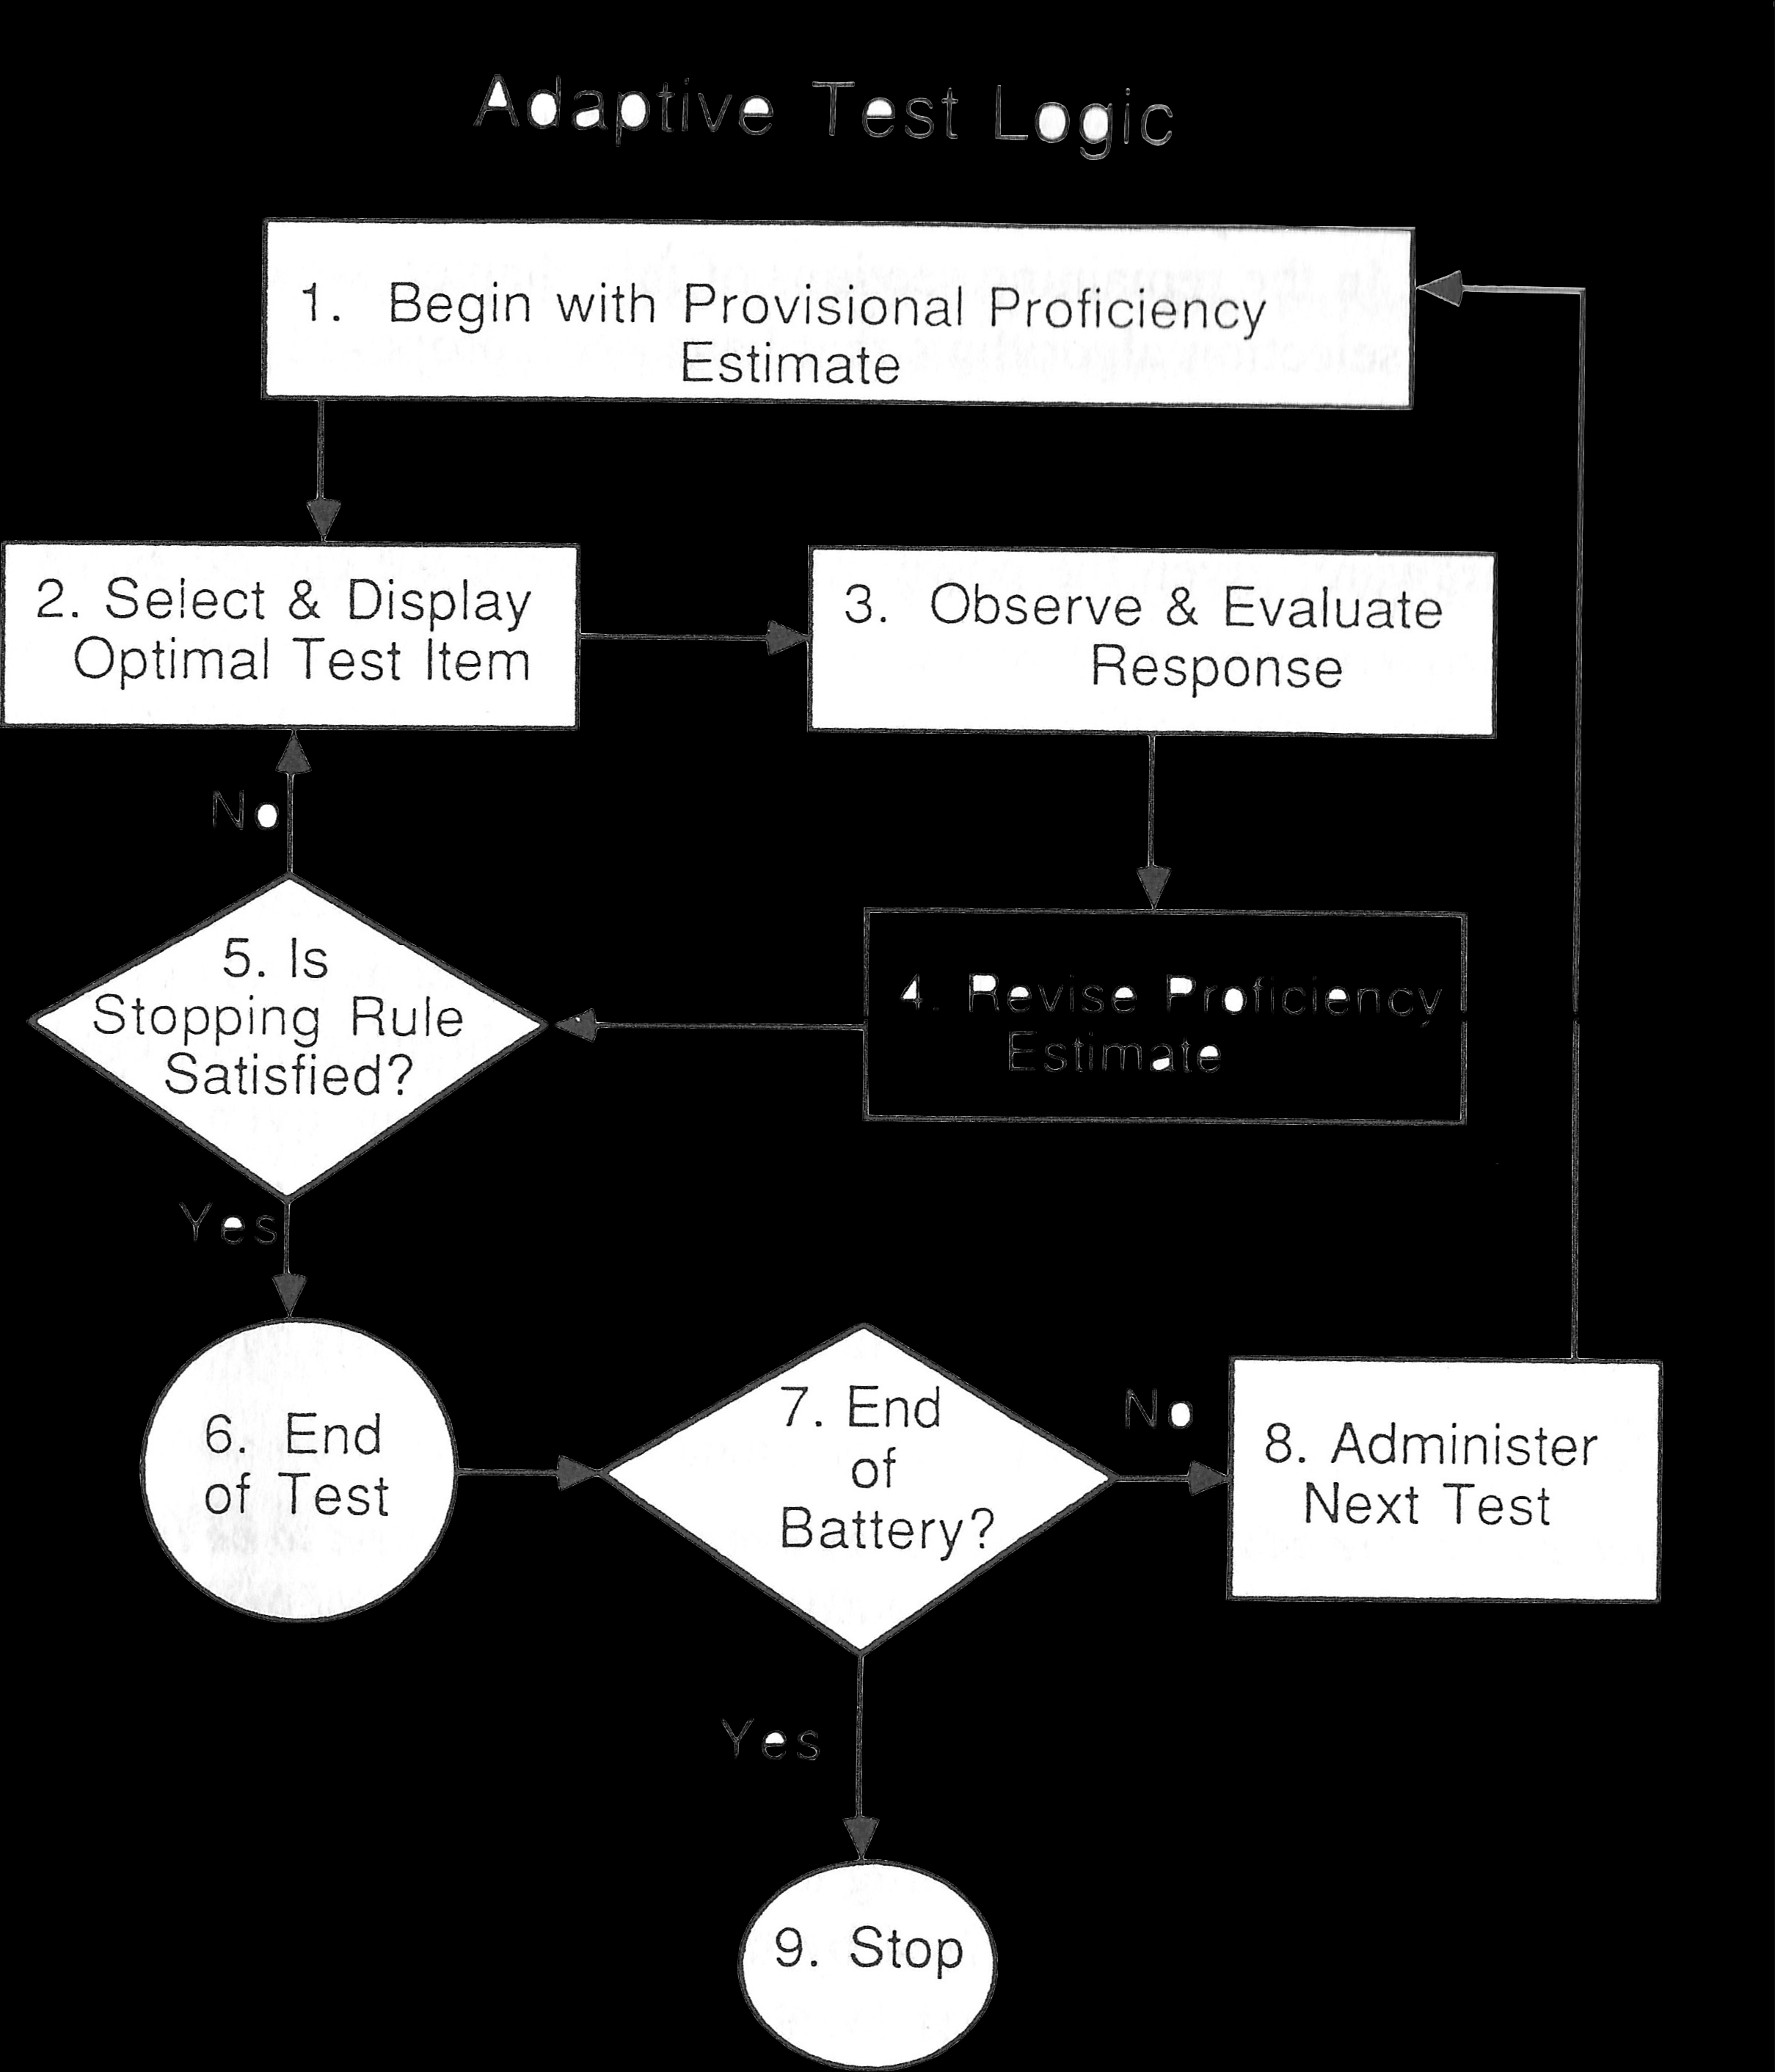
\includegraphics[width=1\textwidth,clip=true]{adaptative_test_logic}
	\caption{Diagrama de flujo de un \acrshort{CAT}}
	\label{fig:diagrama_flujo_CAT}
\end{figure}






In that framework, CAT allows seeing the
students as individuals, taking their own characteristics into
account. Typically, CAT systems are able to adapt the items
presented to the student depending on their former answers, often
including some kind of personalized feedback [12].



Constructing quality test with e-valUAM

Technology-Enhanced Learning (TEL) has a growing presence in educational institutions by making use of Computer-Aided Learning (CAL): a keynote practice where teachers and students are assisted by computers in their teaching/learning processes. Under this perspective, the assessment process is one of those issues that can get profit from the use of these practices. Moreover, completely on-line learning environments, like the emergent trends in Massive Open Online Courses (MOOCs) [1], demonstrate the importance of using CAL environments.

In this context, learning systems, which provide any kind of immediate feedback to students, look to be more effective than traditional learning strategies [2]. We can find in the literature several examples of assessment tools for some specific learning domains that can give useful and interactive advices to the students [3] [4] [5] [6]. In the context of providing feedback and advice to the students for widespread domains, Computer Adaptive Testing (CAT) provides advantages apart from an instantaneous scoring [7]. 

In spite of the advantages of this methodology, items can be inadequately developed by being wrongly classified on a topic or not clearly written up, which can lead to poor quality tests. This situation leads to face an important issue: the need of pre-calibrating test items before they can be used. Usually, a good calibration process implies that the test should be performed by a large population sample [12]. Nevertheless, since the pre-calibration is not always feasible, student models are applied in order to refine the quality of the assessment strategy [19] [20] [21] [22].